\chapter{Background}
The problem space we explore ties together work across a number of different disciplines, including graphics, graphic design, and machine learning modeling.
In hoping to apply generative methods to vectorized glyphs, we are inspired by previous work in computer vision on non-natural images and draw upon recent developments in generative modeling of line drawings.

\section{Non-natural images}
While natural images are photographs of real-world scenes and objects, non-natural images are computationally generated, either by hand with a computer design tool or automatically.
Images in this category include graphs, pictograms, virtual scenes, graphic designs, and more.
Algorithmically understanding, summarizing, and synthesizing these images pose unique challenges because of the images' clean and deliberately drawn designs, sometimes multimodal nature, and human-imbued intent. 

While much attention has been focused on research problems like object recognition, scene segmentation, and image recognition on natural images, interest in applying computer vision methods to non-natural images has been growing.
Much progress has been made towards computationally understanding non-natural images on datasets including XML-encoded scenes~\cite{wu2017neural}, comic strips~\cite{iyyer2016amazing}, and textbook diagrams~\cite{seo2014diagram}.
Recent work by our group has explored the space of infographics, complex diagrams composed of visual and textual elements that deliver a message~\cite{bylinskii2017understanding}.

\subsection{Font faces}
Within the space of non-natural images, we focus specifically on designer-crafted font faces.
Fonts are used to typeset text with particular styles and weights, and many types of fonts exist, including serif, sans serif, and handwriting style fonts.
In this work, our computational methods are applied to font faces downloaded from Google Fonts\footnote{Downloaded from \url{https://github.com/google/fonts}, a GitHub repository containing all fonts in the dataset.}. In Figure~\ref{fig:input_fonts}, a sampling of glyphs from the Google Fonts dataset is shown.

Within a font face, glyphs generally share the same style in properties like angles, curvature, presence of serifs, and stroke width.
In the context of computational modeling and generation, font glyphs offer certain advantages and pose distinctive challenges when compared to other types of designed graphics.
Unlike more complicated designs such as infographics and diagrams, they can essentially be represented as drawings composed of simple lines and curves and, as such, can be modeled using sequential drawing commands.
However, font glyphs have distinct classes (i.e.\ each letter, number, symbol, etc.\ is a different class) and thus designing a generation procedure that is able to create clearly defined instances of different classes presents a difficult problem.

\begin{figure}[]
	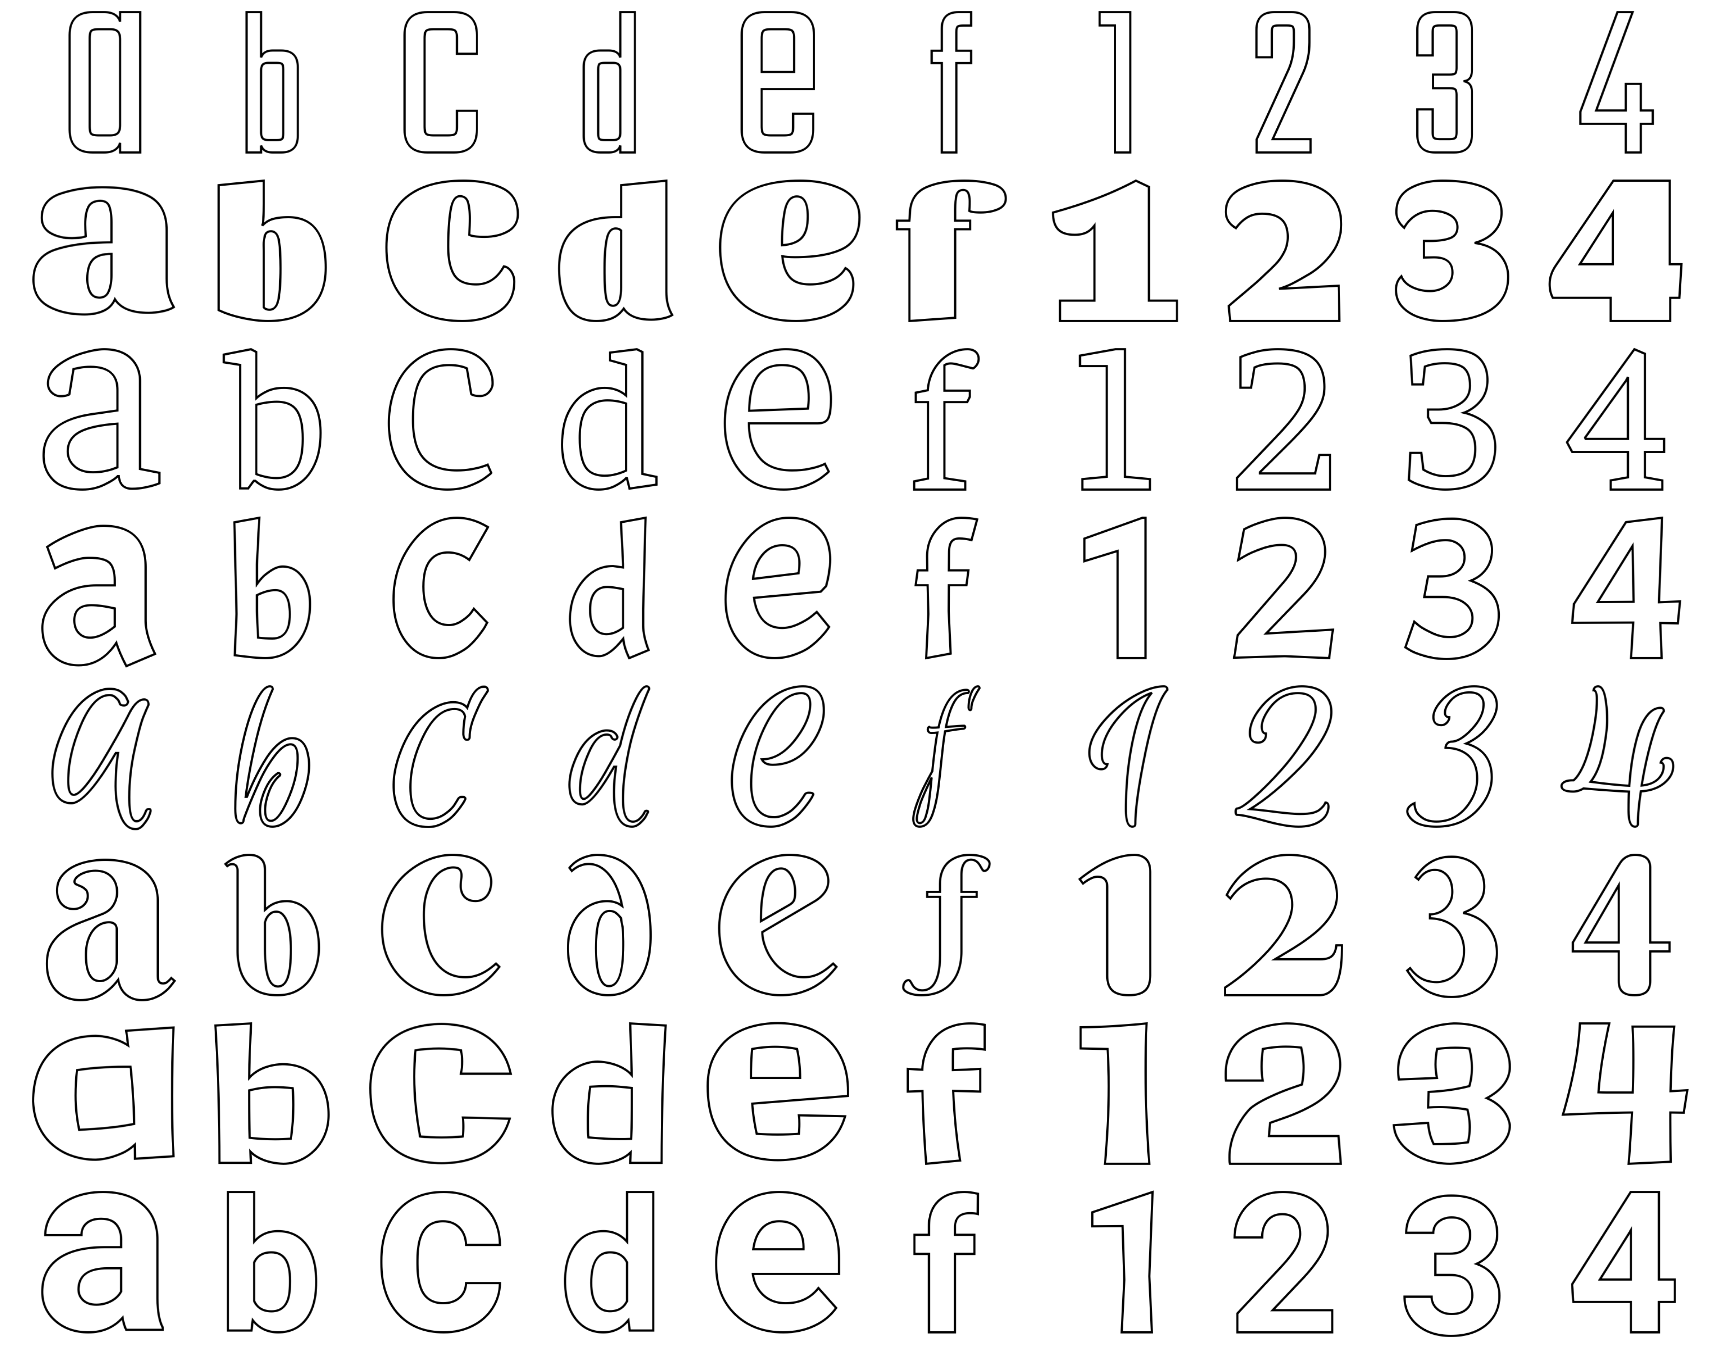
\includegraphics[width=\textwidth]{figures/input_fonts}
    \caption[A sample of the types of font faces used in our fonts dataset]{A sample of the types of font glyphs used in our dataset. Lowercase letters ``a'' through ``f'' are shown, as well as digits 1 through 4. Note the variety of styles represented: the dataset includes serif, sans serif, display, and handwriting style fonts.\label{fig:input_fonts}}
\end{figure}

\subsection{Vector graphics}
In this work, we are primarily interested in applying computational models to vector graphics as opposed to raster images.
While raster images encode color values for each point (or \textit{pixel}) in a two-dimensional grid, vector graphics describe a set of curves and shapes parameterized by mathematical equations and control points.
Many specifications exist for describing images in vector format, including Scalable Vector Graphics (SVG), Encapsulated PostScript (EPS), and Adobe PDF\@.
Font faces are often distributed as TrueType (TTF) files, which encode line and curve commands as well as font hints to aid with rendering.

Although the focus of our research is on font glyph inputs, our vision is to build a generalizable system for the variety of vector graphics generated by designers.
Thus, our system accepts SVG data as input, as most vector graphics formats (including TTF) can be expressed using the commands available in the SVG specification.

Applying computer vision techniques to vector graphics raises new challenges.
While bitmap and vector data can both decode into the same image as viewed by humans, their underlying structures have vast differences (Figure~\ref{fig:svg-a}).
As a data format, SVGs describe lists of geometric objects (among other elements), including lines, circles, polygons, and splines.
The SVG \code{path} element, in particular, can be used to create all other element shapes.
Its attributes describe a series of commands that move from point to point, drawing curves or lines between them, as shown in Figure~\ref{fig:svg-b}.

\begin{figure}[t]
    \subcaptionbox{Raster images are defined as two-dimensional arrays of pixel values, while vector graphics define curves and paths mathematically. Thus, when scaled, vector graphics (right) can still be rendered smoothly while raster images (left) degrade in quality.\label{fig:svg-a}}{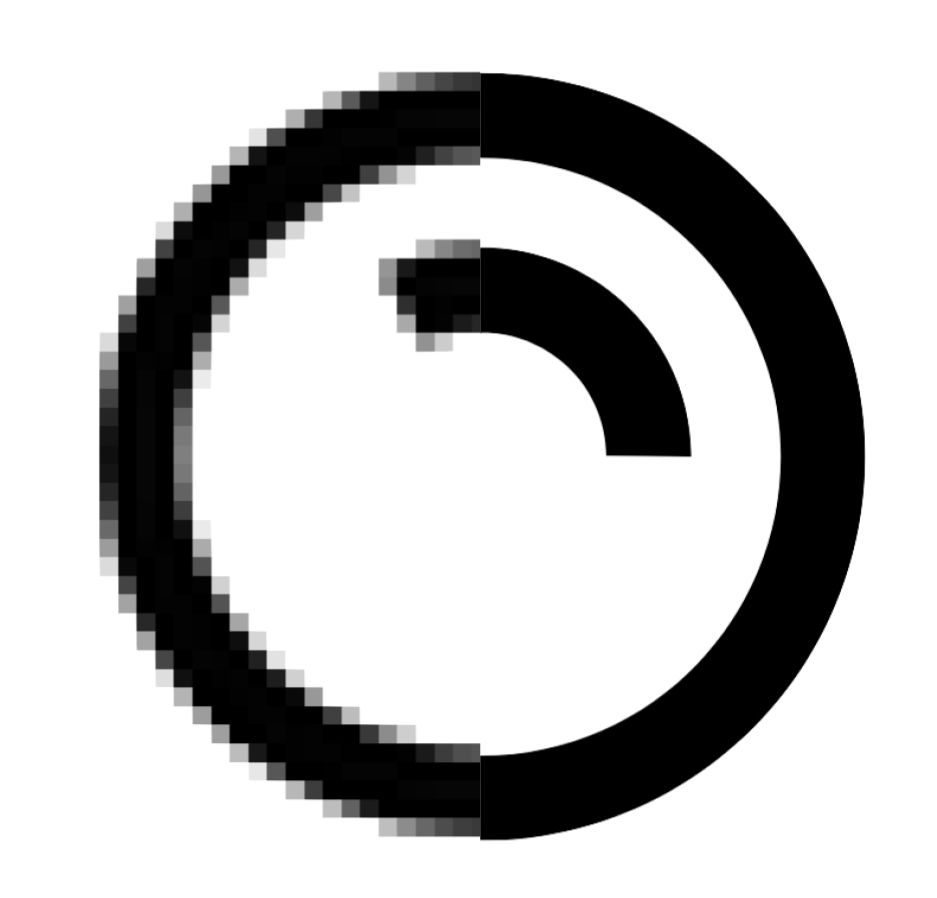
\includegraphics[height=1.85in]{figures/b_vs_vec}} \quad
    \subcaptionbox{SVG is an XML-based markup language that describes geometric elements within a vector image. A single path is used to draw this soap bubble, and colored curves in the image correspond approximately to the highlighted attribute commands that describe them. For example, the command \code{l-0.69-1.32} indicates a line drawn from a starting point to a point 0.69 units to the left and 1.32 units down.\label{fig:svg-b}}{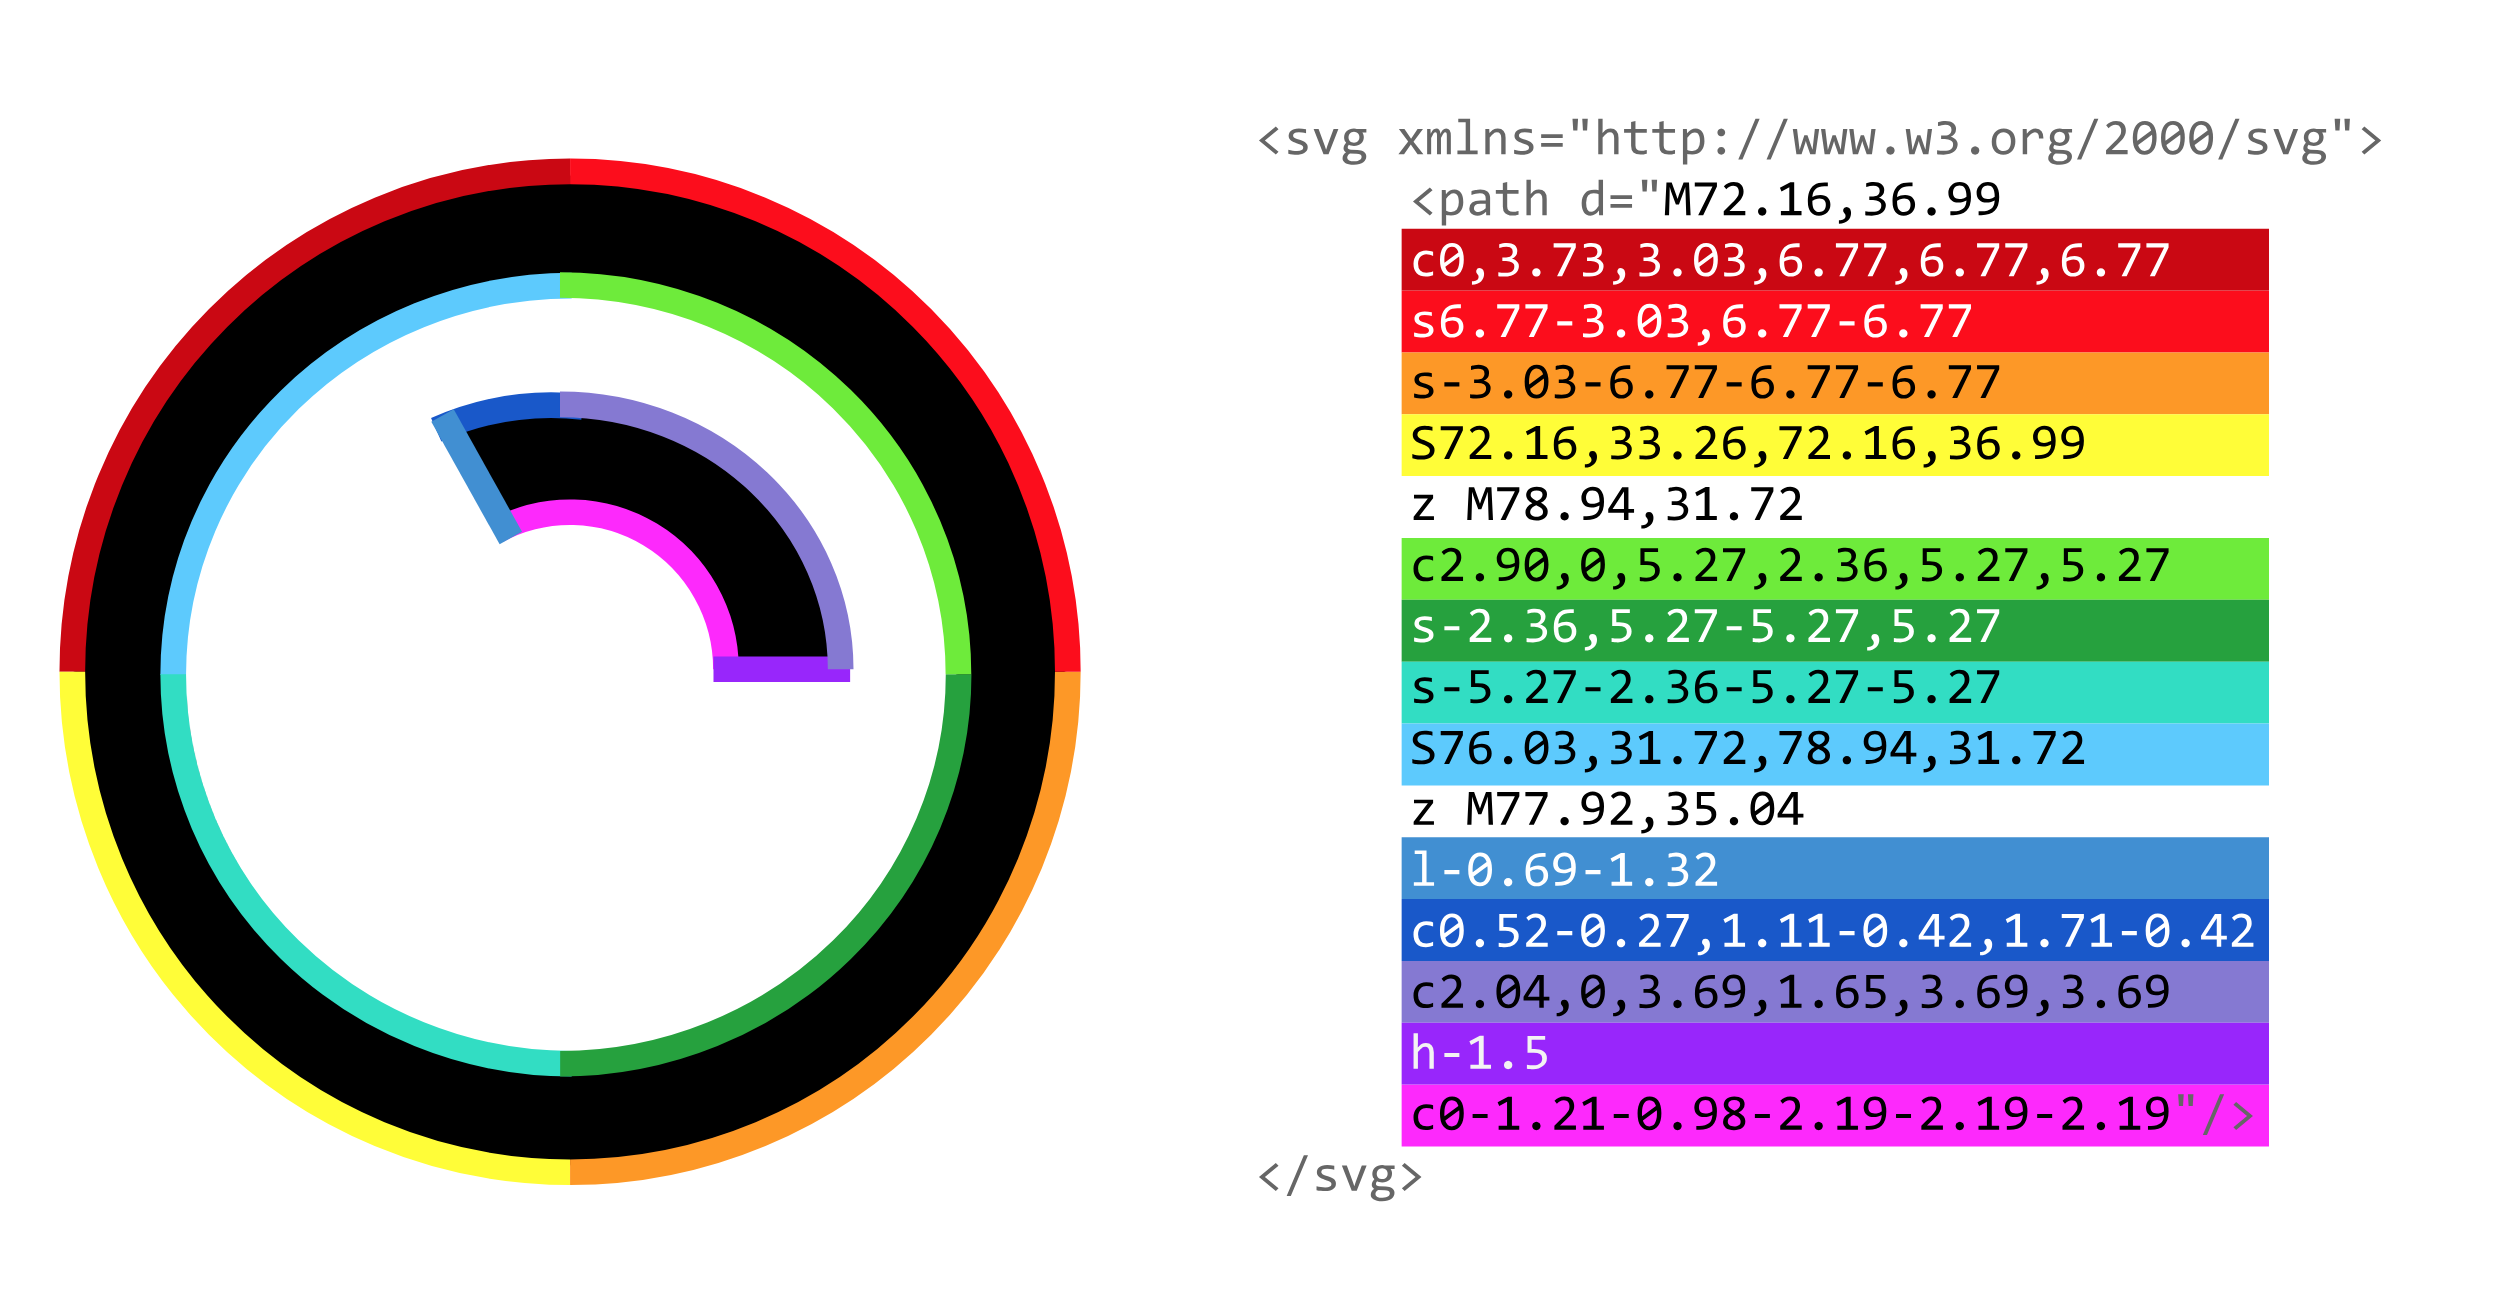
\includegraphics[height=1.85in]{figures/svgs}}
    \caption[An overview of the specification for scalable vector graphics (SVG)]{a visual comparison of raster and vector graphics. Figure~\ref{fig:svg-b} walks through a sample vector graphics path. Image source: \textit{Dog Wash} by Llisole from the Noun Project.\label{fig:svg}}
\end{figure}


\section{Generative modeling}
To solve the problem of creating novel vector drawings, we look towards the tools provided by generative machine learning methods.
While discriminative modeling techniques focus on separating and identifying inputs to produce output labels learned from high-dimensional data such as images, generative algorithms create previously unseen instances of a class based on representative inputs.
They are trained in an unsupervised or semi-supervised manner to model a data distribution $P$, estimating the true data distribution $P_{gt}$ from which samples are drawn.
By drawing probabilistically from $P$, they can then be used to synthesize novel, unseen examples similar to input data.

Two popular neural network-based approaches include generative-adversarial networks (GANs)~\cite{karpathy2016generative} and variational autoencoders (VAEs).
Introduced in~\citeyear{goodfellow2014generative}~\cite{goodfellow2014generative}, GANs pit a generative model $G(z; \theta_g)$ against an adversary $D(x; \theta_g)$ that learns to discriminate samples from the ground truth dataset and the generative model's latent space.
When both models are differentiable functions, backpropagation can be used to train $G$ and $D$ towards convergence in a computationally efficient manner.

\subsection{Variational autoencoders}
Variational autoencoders, introduced in~\cite{kingma2013auto}, explicitly learn an encoder function mapping training examples from the input space $\mathcal{X}$ to a latent space $\mathcal{Z}$ as well as a decoder function mapping from $\mathcal{Z}$ to data points that are in $\mathcal{X}$ but distinct from training inputs $X$.
\TODO{explain more VAE math}

In our work, we specifically build upon the variational autoencoder method in~\cite{ha2017neural}.
\TODO{explain VAE + RNN}

\section{Related work}
\subsection{Image generation}
- DRAW
- SPIRAL
- UToronto handwriting generation
\subsection{Font style}
- Learning a Manifold of Fonts
